%
%  nietzsche.two
%
%  Created by Mark Eli Kalderon on 2008-01-28.
%  Copyright (c) 2008 Mark Eli Kalderon. All rights reserved.
%
%  Beamer

% Definitions and macros
\newcommand{\change}{\textcolor{blue}{\textbf{CHANGE SLIDE}}}
\newcommand\myauthor{Mark Eli Kalderon} 
\newcommand\mytitle{Introduction to Moral Philosophy}
\newcommand\mysubtitle{Nietzsche}
\newcommand\myinstitution{University College London}
\newcommand\myurl{http://markelikalderon.com/teaching}

% Packages specific to lecture notes
\mode<article>{
    \usepackage{palatino}
    \setjobnamebeamerversion{nietzsche.two.beamer}
}


% Packages specific to beamer presentation
\mode<presentation>{
    \usetheme{Darmstadt}
    \setbeamercovered{transparent}
    \pgfdeclareimage[height=0.5cm]{university-logo}{../../../graphics/logo_sml_blk}
    \logo{\pgfuseimage{university-logo}}
}

% Packages common to lecture notes and beamer presentation
\usepackage{pgf}
\usepackage{tikz}
\usepackage{hyperref}

\title{\mytitle}
\subtitle{\mysubtitle}

\author{\myauthor\\
\url{\myurl}}
\institute{\myinstitution}

% \date[Short Occasion] % (optional)
% {Date / Occasion}

\begin{document}

\frame{\maketitle}

\section{Review}\label{sec:review} % (fold)

Two questions form the basis of the \emph{Genealogy}:
\begin{itemize}
    \item What is the value of (our) moral values?
    \item What are the conditions and circumstances that give rise to these values?
\end{itemize}
Two observations were relevant to making sense of the first question. First, we observed that Nietzsche was appealing to the Aristotelian insight that conforming our actions to the dictates of morality ought to promote human flourishing. The Aristotelian insight gives us a measure of the value of our values. Our values are only valuable insofar as the promote human flourishing. We saw how Nietzsche has an idiosyncratic conception of human flourishing---human flourishing consists in great concentrations of and consciousness of will to power. So our values are valuable only to the degree to which they promote or hinder concentrations or consciousness of will to power. Second, we observed that for Nietzsche, morality was a family of resemblance concept---that there are no necessary and sufficient conditions for a given practice to count as a morality. Rather there are overlapping patterns of resemblance that obtain between diverse practices in virtue of which they all count as moral practices. Sometimes when Nietzsche speaks of morality he means one of the particular historically conditioned practices that belong to the family of resemblance sometimes he means morality more generally. So when Nietzsche describes himself as an immoralist he means morality in the specific sense, that is, Nietzsche is an immoralist from the perspective of the Christian morality he rejects as a positive hindrance to human flourishing. 

The project of determining the conditions and circumstances that give rise to these values is contrasts with a pedigree. In contrast with a pedigree, the function of a genealogy is not to legitimize or positively valorize Christian moral practice, indeed the genealogy of morality will be the basis of its criticism. Whereas a pedigree begins with a singular origin, morality is the result of diverse lines of development. With a pedigree, the singular origin is the source of the value. However, with a genealogy, the further back it is pursued the less likely we will discover something we value. Whereas a pedigree uncovers a linearly ordered sequence of events, the events involved in a genealogy have a tree-like structure. Finally, the steps in a genealogy do not transmit value the way that the steps of a pedigree do, rather they \emph{institute} value. \change

\begin{frame}<presentation>[label=slide1]
    \frametitle{Review}
        \begin{columns}
            \begin{column}{3cm}
                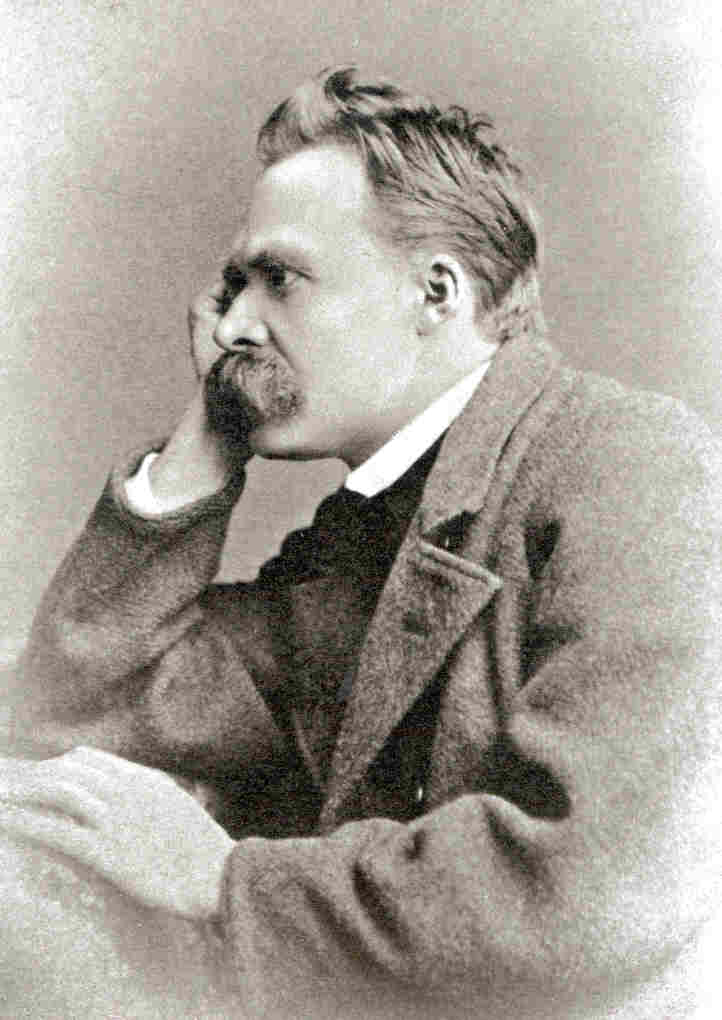
\includegraphics[height=4cm]{../../../graphics/nietzsche.jpg}
            \end{column}
            \begin{column}{7cm}
                \begin{itemize}
                    \item What is the value of (our) moral values?
                    \item What are the conditions and circumstances that give rise to these values?
                \end{itemize}
            \end{column}
        \end{columns}
\end{frame}

Now that we have gotten somewhat clearer on the two central questions of the \emph{Genealogy}, let us consider their interconnection. What is the relationship between the value of our values and the historical circumstances that gave rise to them. How can genealogical inquiry provide us with the resources to determine the value of our morality? A complete answer to this question will not be unavailable until we discuss the third essay of the \emph{Genealogy}. But for now,let's consider what this relation could not be.

Nietzsche, in insisting that the history of our morality is relevant to determining its value, comes perilously close to committing what is known as the \emph{genetic fallacy}. The genetic fallacy is the conflation of the value of something with the value of its origin. Just because something has some value it does not follow that it came about on account of the value it now possesses. 
\begin{quote}
    \emph{The Genetic Fallacy}: the conflation of the origin of a thing with its present value.
\end{quote}

It would seem then that there is no direct inference from the conditions that give rise to a thing to the value it now possesses or vice versa. How then is genealogical inquiry at all relevant to determining the value of our morality? Isn't Nietzsche's project simply confused at the outset---an ill advised enterprise initiated by a non-rigorous thinker?

We should caution against such a hasty dismissal of Nietzsche's project. Nietzsche himself is under no illusion as to the genetic fallacy. Nietzsche explicitly identifies such a fallacy in his book \emph{Daybreak} where he writes:
\begin{quote}
    more insight we possess into an origin the less significance does the origin appear... 
\end{quote}
Not only does he explicitly recognize the genetic fallacy, but he criticizes previous genealogists for committing just this fallacy. In particular he objects to the kind of genealogy of morality provided by English psychologists precisely because it conflates the origin of our morality with its value:
Originally---so they decree---one approved unegoistic actions and called them good from the point of view of those to whom they were done, that is to say those to whom they were useful.; later one forgot how this approval originated and, simply because unegoistic actions were always habitually praised as good, one also felt them to be good---as if they were good in themselves.

Nietzsche maintains that it is a psychological absurdity that the original utility of unegoistic actions has been forgotten: this utility has rather been an everyday experience at all times, therefore something that has been underlined again and again: consequently instead of fading from consciousness, instead of being merely forgotten, it must have been impressed on the consciousness more and more clearly. Not only is this account psychologically suspect, but it is historically suspect as well. The English psychologists infer from the present utility of valuing unegoistic actions to such valuations arising because of their utility. Indeed, Nietzsche maintains that the opposite is true. Originally the concept good did not designate unegoistic actions. It is only because the English psychologists did not pay careful enough attention to the historical record that they were seduced by the genetic fallacy.

Nietzsche thus not only recognizes the existence of the genetic fallacy but also recommends the rigorous application of historical methods as a preventative. It would thus be uncharitable in the extreme to simply accuse him of making just this mistake. Rather, the fact of his explicit recognition of the genetic fallacy forces us to consider whether the argument of the \emph{Genealogy} is more subtle than this. And indeed I believe it is.

What then is the connection between the genealogy of morality and the determination of its value? Perhaps the connection is this: a careful historiography of morality will reveal whether and to what extent Christian morality has hindered or promoted human growth and vitality so far. The fact that Christian morality has so far hindered or promoted human flourishing surely provides us some good evidence as to whether it presently hinders or promotes ``the growth of the plant `man''' To be sure the historical record provides some evidence but such evidence is far from conclusive. Just because some value or system of values has hitherto hindered or promoted human flourishing it does not follow that these values will presently hinder or promote human growth and vitality. Under a given set of contingent, historical circumstances a morality may promote human flourishing and under another set of circumstances it may prove to be a positive hindrance, and vice versa. Nietzsche denies moral values are universal in the sense of themselves being valuable for everyone and everywhere and at all times. As such, he cannot in good conscience maintain that the fact that Christian morality has heretofore hindered or promoted human flourishing is conclusive evidence that it will continue to do so.

So what then is the argument of the Genealogy? How is the genealogical record of morality relevant to determining its value? As I said before, a complete answer to this question must wait until we have discussed Nietzsche's account of the significance of ascetic ideals in the third essay of the book. But let me make a few comments as to its oblique character. One useful way to think about Nietzsche's case is that it is a kind of demonstration. ``Demonstration'' is ambiguous but both of its senses is relevant to the character of Nietzsche's case. In one sense of demonstration, if one has demonstrated some proposition one has established it with the requisite rational authority. Thus we sometimes speak of mathematical proof as a demonstration. In another sense of the word, a demonstration, unlike an argument in propositional form, is explicitly nonpropositional. In this sense, to demonstrate something is to display or show it rather than describing it. Thus we can speak of a golf pro as demonstrating the proper swing after explicitly describing it. Nietzsche's case is a demonstration in something like both these senses. It is supposed to have the rational authority of explicitly recognized forms of argument and yet it is displayed or shown in the style of the text rather than being explicitly argued for in propositional form. Once again, the crucial link is in the third essay so I will simply leave you with these tantalizing remarks until then. However, I hope this underscores the importance of paying careful attention to Nietzsche's style. \change

\begin{frame}<presentation>[label=slide2]
    \frametitle{The Genetic Fallacy}
        \begin{columns}
            \begin{column}{3cm}
                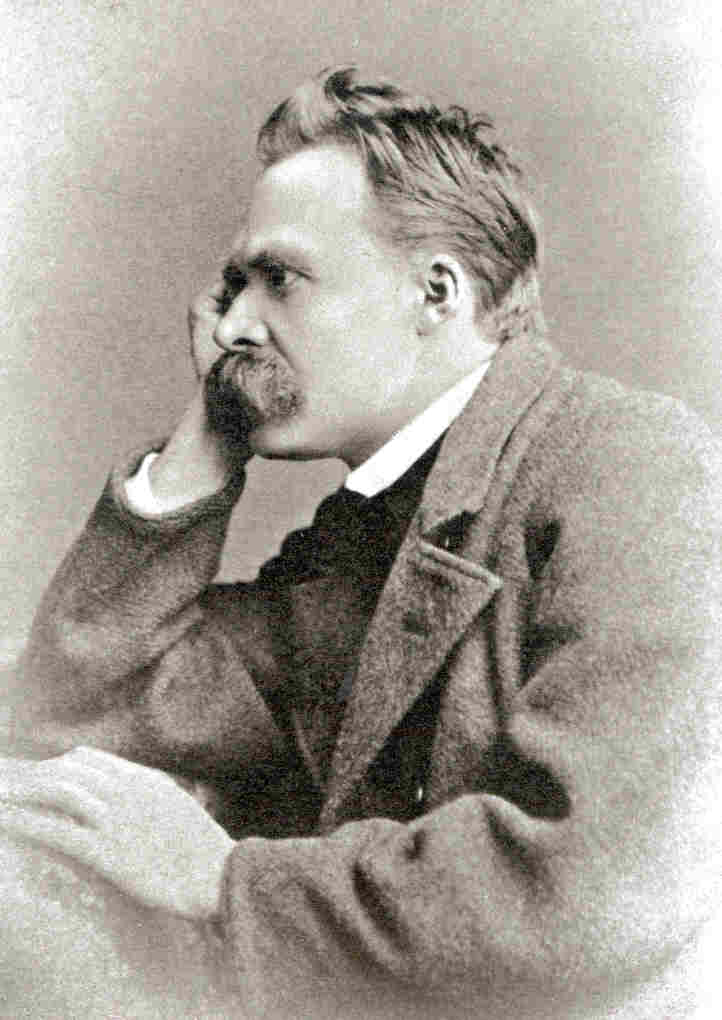
\includegraphics[height=4cm]{../../../graphics/nietzsche.jpg}
            \end{column}
            \begin{column}{7cm}
                \alert{The Genetic Fallacy}: the conflation of the origin of a thing with its present value.
            \end{column}
        \end{columns}
\end{frame}


% section review (end)

\section{Christian Morality}\label{sec:christian_morality} % (fold)

Before we begin discussing Nietzsche's critique of morality, we should first get a clearer conception of the Christian morality that he opposes. Nietzsche maintains that European morality derived from Christianity is structured by six characteristic theses:
This morality claims of itself that it is unconditional in the obligation it imposes.
\begin{itemize}
    \item It claims to be universal---it applies equally to all human beings at all times and places.
    \item It claims that only free human actions have moral value.
    \item It claims that the moral worth of a free action depends on the quality of the human choice that leads the agent to perform it.
    \item It claims that human beings and their actions are to be evaluated (positively) as  ``good'' or (negatively) as  ``evil'' depending on the kind of human choice involved.
    \item It claims that we are responsible for our choices and should feel guilt or remorse for evil choices.
\end{itemize}
As will emerge, Nietzsche will taken exception with 19th century Christian morality on all 6 points.

Like many other religions, Christianity has a bipartite structure: a set of antecedently existing practices, modes of behavior, perceptions, and feelings, which at a certain time are given an interpretation which imposes on them a meaning that they did not have before. Thus in the specific case of Christianity Nietzsche distinguishes a way of life a practice which is specifically associate with the historical Jesus because he is thought to have instantiated it to a particularly high degree and in a particularly striking way, but which is in principle livable almost anywhere and anytime, a form of life, of instinctive practice, not a form of belief, which consists on the unconditional forgiveness of enemies, a failure to resist evil, abstention from use of force or the moral condemnation of others from a particular interpretation put on that way of life (as instantiated by Jesus), that is, a set of propositions that eventually become the content of Christian faith and belief. This interpretation is more or less invented by Paul and contains various dogmatic propositions about the existence of God, the immortality of the human soul, human sinfulness and the need for redemption. Though Paul did succeed in getting his reading of the meaning of Jesus accepted his dogmas did not fit very comfortably with the original form of practice Jesus instantiated. To be more exact, Paul's interpretation represents so drastic and crude a misinterpretation of Jesus' way of life that even at a distance of 2000 years we can see that wherever the Pauline reading gets the upper hand---and it has in general had the upper hand for most of the period in question---it transforms Christianity (as we can now call the amalgam of Jesus way of life and Paul's interpretation of it) into what is the exact reverse of anything that the historical Jesus would have praticed. An essentially a political, pacifist, non-moralizing form of existence is transformed into a Church a hierarchically organized public institution---just the thing Jesus preached against.

Paul's interpretation of Jesus's life (which forms the core of Christian theology) is wrong in two ways. First of all it is a misunderstanding of Jesus's way of life. For Paul, Jesus' life and death essentially has to do with sin and redemption, but the message of Jesus' life really is that there is no sin and that the very concept of guilt has been abolished. Second Paul's propositional beliefs taken by themselves (and not necessarily as an interpretation of the life of Jesus) are false. For Nietzsche the whole notion of sin is in its origin a priestly misinterpretation of certain physiological states of debility and suffering and the concept of guilt in the full blown Christian sense depends on the false assumption that humans have freedom of the will and can thus decide to exercise or refrain from exercising the various powers they have.

Paul's hijacking of the form of life as embodied by Jesus is one episode in what Nietzsche calls the genuine history of Christianity, but it shows in particular clarity the bipartite structure (of  ``form of life '' on the one hand and  ``interpretation '' on the other) which was mentioned earlier. It is important to see that Paul's successful attempt to take over the Christian form of life by reinterpreting it is only one of a number of such episodes. Each such attempt can be described as at the same time a new interpretation of Christianity as it exists at the given time and as an attempt to take over or get mastery of that existing form of Christianity. Each historically successive interpretation gives the existing Christian way of life a new meaning.

Although Nietzsche at one point says that Paul annuls original Christianity this doesn't mean that Paul wishes to abolish wholesale the practices that constitute this primordial form of Christianity. Rather he wants to impress on them a stamp of a certain meaning, give them a certain direction. Nietzsche thinks that such attempts to take over/reinterpret an existing set of practices or way of life will not in general be so successful that nothing of the original form of life remains, hence the continuing tension in post-Pauline Christianity between forms of acting, feeling, judging which still somehow eventually derive from aboriginal Christianity and Paul's theological dogmas. Equally once Paul's reading of Christian practice has given these practices a certain meaning, the historically next reinterpretation will in turn find the Pauline meanings already embedded in the form of life it confronts and will be unlikely in giving a new interpretation of that form of life to abolish the Pauline concepts and interpretations altogether. Historically, then, successive layers of such meanings will be deposited. There will be some gradual change in the actual practices and form of life---Pauline Christianity will begin to develop a Church organization which primordial Christianity lacked, but even the dominant interpretation won't have been able utterly to eradicate the meanings that have previously accumulated, that have been impressed upon Christianity by previous wills.

The history of Christianity, then, is a history of successive attempts on the part of a variety of different wills to take control of and reinterpret a complex of habits, feelings, ways of perceiving and acting, thereby imposing on this complex a meaning. Although the meaning imposed at any time by successful will may in some sense be superseded by a later meaning imposed by a later will, the original meaning will in general not go out of existence altogether but will remain embedded in at least a modified form in the complex we call Christianity. Part of the reason for this is that once a certain will has been able to impose its meaning on Christianity, it acquires a certain power of resistance to any further attempts on the part of other wills to impose their meaning on the Christian complex. Once Pauline theology has penetrated Christian practice, modified it, given it a certain direction and a particular kind of coherence etc. any non-Pauline will which tries to impose a new interpretation on Christianity (as thus constituted) won't encounter, as it were, just a tabula rasa, but a set of actively structured forces, practices, etc. which will be capable of active resistance to attempts to turn them into other directions, impose new functionson them, etc. So each episode of reinterpretation will be a struggle between a will impinging from without bent on mastery attempting to impose of a new meaning and a complex way of life which will resist at least by inertia and evasion and probably by more active measures as well.

Christianity at any given point of time will be a synthesis of the various different meanings imposed on it in the past and which have succeeded in remaining embedded in Christian feeling, forms of action and belief, etc. There will be nothing necessary nor even particularly coherent about such a synthesis---what meanings it will contain and how they will be relate to one another will just be the result of history, and this history will be contingent in a number of different ways. It will be contingent which wills will encounter and try to master and interpret Christianity at what times and under what circumstances, and it will be contingent how much force, energy, and success they will have in imposing their meaning. The history of Christianity will, as Nietzsche writes in the section 13 of the second essay of the Genealogy,  crystallize itself into a kind of unity which is difficult to dissolve, difficult to analyze, and, it must be emphasized, utterly undefinable.

One can't give a definition of Christianity if one means by that an account of a purported or essential meaning (or purpose or function) which is invariably characteristic of Christianity. Nietzsche claims that only that which has no history is definable because anything that has a history will partake like Christianity in the continuing struggle between wills attempting to impose their meaning or purpose on the item in question, a struggle with constantly shifting outcomes. Instead of a definition, one must try to give a historical analysis of the contingent synthesis of meanings Christianity, for instance, represents. This process of disentangling the separate strands will take the form of a historical account. The reason for this seems to be that  at an earlier stage the synthesis of meanings presents itself in such a way as to be more easily dissolved. The individual elements are more distinct.

The appropriate historical account is a genealogy. Starting from the present state of say Christianity or whatever else is the object of genealogical inquiry the genealogy works backwards in time, recounting the episodes of struggle between different wills, each trying to impose its interpretation or meaning on the practice that existed at that time, and thereby disentangling the separate strands of meaning that have come together in a contingent unity in the present. Each such episode is, as it were, the branching node of a genealogical tree---the kind of tree represented by the diagram I gave you last time. The diagram was intentionally just a sketch of Nietzsche's account, leaving out many details in order to exhibit more clearly the overall structure. At various points the branches simply end but those endpoints are not absolute origins. The genealogy peters out there either because there is not more information available or because further elaboration of the genealogy at that point would lead too far afield, but in principle if the information were available and there was reason to continue, one could carry the genealogy back beyond the points at which Nietzsche in facts stops.

This is true in particular for the end-point I designated Jesus' radically non-moralizing from of life. I said earlier that religions for Nietzsche generally have a bipartite structure: a particular way of living on the one hand and an interpretation of it on the other. In this case, there is Jesus' way of life and Paul's interpretation of it, and only both together constitute what we call Christianity. One might think that having thus recognized the difference between Jesus and Paul we could now strip back the Pauline interpretation and we could get back to something that was not interpretation but the way of life in itself, a final stopping point, and absolute origin. That one can get back to the thing itself, unvarnished and uninterpreted is an illusion. Unless one believes in miracles, Jesus' practice itself has historical antecedents that could be genealogically analyzed. In addition Jesus' way of life, although it is not constituted by explicit belief in a set of propositions of the kind Paul asserts, can be itself seen as a kind of interpretation. For Nietzsche, I am interpreting a situation by reacting to it in a certain way. If I recoil from it, I am interpreting it as repulsive; if I draw near it I am interpreting it to be attractive; if I pass by without reacting to it at all, I am treating the situation as irrelevant or insignificant. This is, presumably, one of the things that Nietzsche means when he claims that life itself is a process of evaluating and giving preferences. So Jesus' form of life, although not characterized by explicit theological beliefs of the Pauline kind, will have the same two part structure: it will ultimately show itself as arising from an episode in which certain will with a certain interpretation of things tries to take over a preexisting form of life (although this interpretation now won't, as in the later Pauline case, be essentially a question of affirming or believing propositions, but of acting, feeling, and perceiving in a certain way). I can't tell you what Nietzsche thinks this antecedently existing mode of living (which Jesus took over and reinterpreted) was, because he doesn't say, but in the \emph{Genealogy} Nietzsche claims that Jesus' good news of universal love was not the reverse of Jewish hatred but grew out of it as its crowning achievement. It would be mistake I think, to interpret this as meaning that Jesus' love was not really love but rather really hate. It would also be a mistake to identify this transformation of hate into universal love in the person of Jesus with what Nietzsche calls the slave revolt in morality, the transformation of the valuations based on the contrast good/bad into a valuation based on the contrast good/evil. Paul is a central figure in the slave revolt which lies in the main line of development of modern western morality; Jesus on the other hand was for Nietzsche only very marginally associated with the genesis of our morality. Both arise out of the deepest and most sublime hatred that ever was on earth, but each transforms this hatred in a completely different direction: Paul into a form of guilt ridden, moralizing asceticism, and Jesus by becoming virtually a ``free spirit'' a man incapable of negating or refuting with no conception of sin, guilt or punishment. When Nietzsche sums up his campaign against traditional morality, the formulation he uses is not Dionysos against Jesus but Dionysos against The Crucified. The crucified being, of course, the name of the Pauline God.

Let me make one more comment on the relationship between determining the value of our morality and undertaking its genealogy. Given Nietzsche's historicist conception of meaning, that the meaning of an institution or practice is ultimately constituted by the various wills that have sought to master and interpret it, genealogical inquiry is one sense clearly relevant to the project of determining the value of our morality. For the content of our present morality, the synthesis of the various meanings that it has come to embody through its long history, can only be determined by undertaking the kind historical inquiry that Nietzsche recommends. That is, before we can determine the value of our morality we must have a clearer conception of its content, and in order to do that we must first undertake its genealogy. While the content of our morality, as revealed by genealogical analysis, is relevant to determining its value, the degree to which it promotes or hinders human growth and vitality, genealogy still cannot by itself answer the initial question as to its value. So while Nietzsche's interpretivism, that the meaning of thing is an interpretation imposed on it by a will from without, definitely sheds light on the relevance of genealogy to the question of the value of our morality, it is still unclear whether and how and answer to the genealogical question can be a sufficient basis for determining the value of our moral practice. \change

\begin{frame}<presentation>[label=slide3]
    \frametitle{Christian Morality}
        \begin{itemize}
            \item It claims to be universal---it applies equally to all human beings at all times and places.
            \item It claims that only free human actions have moral value.
            \item It claims that the moral worth of a free action depends on the quality of the human choice that leads the agent to perform it.
            \item It claims that human beings and their actions are to be evaluated (positively) as  ``good'' or (negatively) as  ``evil'' depending on the kind of human choice involved.
            \item It claims that we are responsible for our choices and should feel guilt or remorse for evil choices.
        \end{itemize}
\end{frame}

% section christian_morality (end)

In the first essay Nietzsche seeks to uncover the natural (as opposed to supernatural) conditions that gave rise to the concepts of good and evil and the associated forms of moral valuation. The dark unchristian truth uncovered by this initial genealogical inquiry is that the moral distinction between good and evil is not divinely sanctioned but is rather the result of what Nietzsche describes as the slave revolt in morality. The slave revolt depends on a number of contingent historical episodes. In particular, the existence of pre-moral aristocratic societies whose rank ordering gave rise to rank defining pre-moral form of valuation deploying the distinction between good and bad, that a certain ruling group divides itself internally into military faction and a priestly faction, that the priestly subcaste begins to use terms of ritual purity to differentiate itself and eventually loses out in a power struggle with the military subcaste, that the priests decide to make common cause with the slaves who happen to speak a language which makes the grammatical distinction between subject and predicate, that the slaves form a novel form of valuation based on the spirit of \emph{ressentiment} features of which are crucially influence by this grammatical feature and which designates as good all that the noble form of valuation deemed bad, and evil all that the noble form of valuation deemed good. All of these events are thouroughly contingent, they could have gone otherwise. The origin of good and evil is an accident of history not further susceptible to any kind of deeper explanation.

The first essay begins with Nietzsche's criticism of his genealogical predecessors. By his own lights, Nietzsche is not the first to undertake a genealogical inquiry into the moral past of mankind. The so-called English psychologists also approached the moral history of mankind with the requisite naturalism. That is, they attempted to uncover the naturalistic conditions that gave rise to moral phenomena. Though the English psychologists attempted to provide a genealogy of morals, the historiography that they produced was inept lacking, as they were, as Nietzsche puts it, ``the historical spirit''. As we discussed earlier, Nietzsche accuses the English psychologists of committing the genetic fallacy. They observe that unegoistic actions are praised as good and that positively valuing such actions has great utility. From this they infer that unegoistic actions were originally designated as good because of their utility. Thus we have an inference from the present utility of valuing a range of action to their originally being valued because of this utility. But there is no direct inference from the present value of a thing to its origin or vice versa. That is just the genetic fallacy.

Nietzsche not only criticizes previous genealogists for committing the genetic fallacy but he also provides a diagnosis for why they were misled. The temptation to commit the genetic fallacy was the direct result of the failure to pay careful attention to documented historical record. Nietzsche insists that if an adequate genealogy of morals is to be given, one cannot proceed by  ``gazing haphazardly around in the blue.'' Rather  one must pay careful attention to the available historical evidence. Genealogy is a gray science, dedicated as it is to deciphering the long hieroglyphic record of our shared moral past. Nietzsche remarks that he himself only began to make progress when he focused on a particular range of historical evidence, that is, philological evidence. Philology is now more comonly designated as historical linguistics. It is the study of linguistic changes over time in a language or family of languages sometimes even extending to the reconstruction of previous languages now lost. In particular, Nietzsche was struck be a remarkable fact about the history of our moral language---that terms used originally to denote political superiority resolve over time into terms denoting moral superiority. Nietzsche supports this hypothesis through a variety of differect examples culled from different languages of moral terms and their etymological roots. I won't here review the philological evidence that Nietzsche puts forth. But what he discovers is that terms used to mark a distinction of political superiority over time come to denote typical character traits  of the aristocracy which eventually come to have normative significance. \change

\begin{frame}<presentation>[label=slide4]
    \frametitle{Nietzsche and Philology}
        \begin{columns}
            \begin{column}{3cm}
                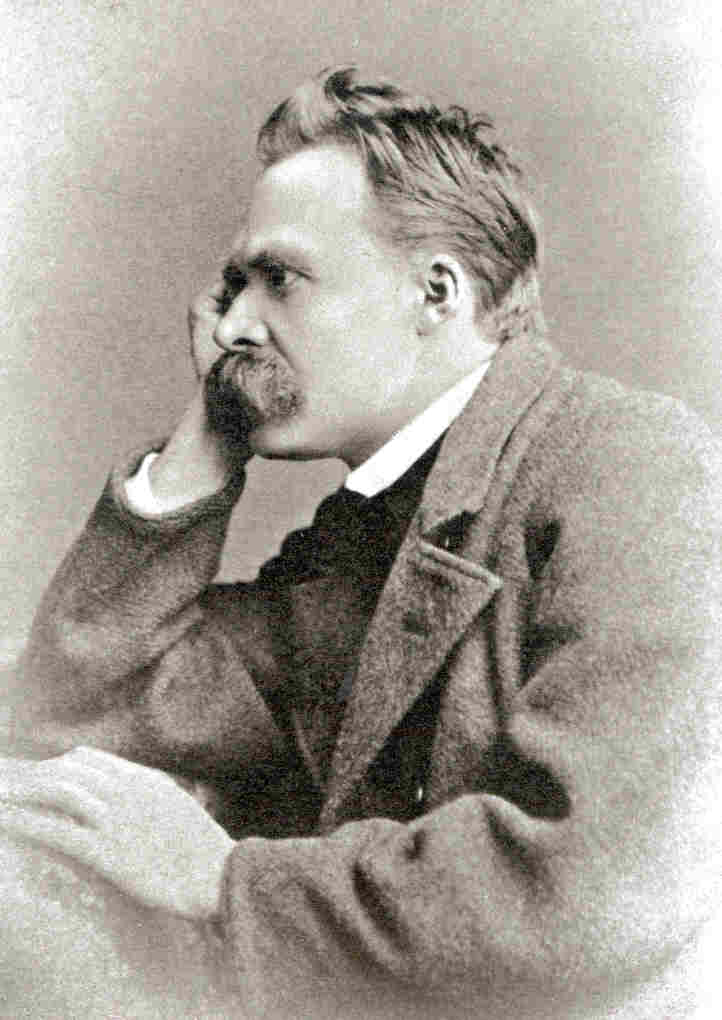
\includegraphics[height=4cm]{../../../graphics/nietzsche.jpg}
            \end{column}
            \begin{column}{7cm}
                \alert{Philology} is a form of historical linguistics---it is the study of linguistic changes in a language or family of languages sometimes even extending to the reconstruction of extinct languages.\\
                \alert{Nietzsche's Fundamental Philological Hypothesis}: Terms used to denote political superiority resolve over time into terms denoting moral or spiritual superiority.
            \end{column}
        \end{columns}
\end{frame}

\section{Pathos of Distance}\label{sec:pathos_of_distance} % (fold)

Nietzsche's philological research thus leads him to discover two things: the general conditions that give rise to values---the pathos of distance---and a pre-moral, noble mode of valuation. The pathos of distance is the long lasting feeling of power of the higher ranks of society. Nietzsche believes that the philological record establishes the hypothesis that the creation of values are always tied to this kind of rank-ordering and consciousness of power. Furthermore, in examining the philological record Nietzsche discovers a pre-moral form of evaluation, the so-called noble form of evaluation that is distinct in content and motivation from the more familiar Christian mode of evaluation. In contrast with the Christian distinction between good and evil, Nietzsche discovers a distinction that predates it, between good and bad, and that involved a fundamentally distinct form of evaluation. In its earliest uses, ``good'' denoted the good themselves that is the noble high ranked who established themselves and their actions as good in distinction from the lowly or plebeian. Nietzsche's fundamental philological hypothesis thus provides empirical evidence for two claims:
\begin{itemize}
    \item novel values always arise out of the ``pathos of distance'' 
    \item there was a noble mode of evaluation involving the distinction between ``good '' and  ``bad '' that predates the Christian distinction between good and evil.
\end{itemize}

\change

\begin{frame}<presentation>[label=slide5]
    \frametitle{Two Discoveries}
        \begin{columns}
            \begin{column}{3cm}
                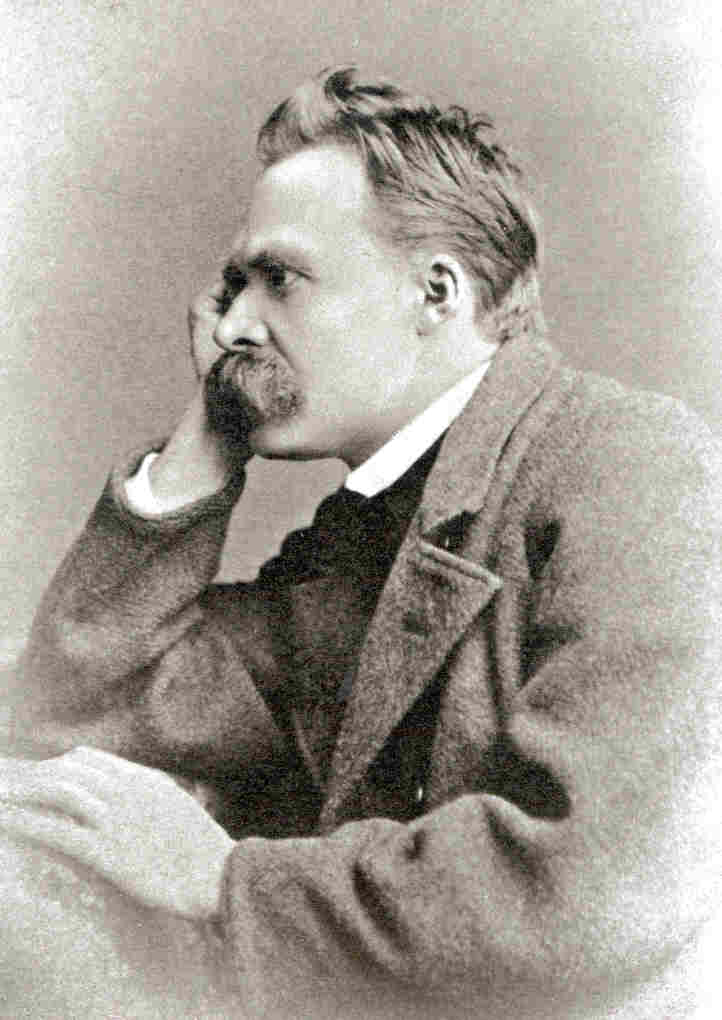
\includegraphics[height=4cm]{../../../graphics/nietzsche.jpg}
            \end{column}
            \begin{column}{7cm}
                \begin{itemize}
                    \item novel values always arise out of the ``pathos of distance'' 
                    \item there was a noble mode of evaluation involving the distinction between ``good '' and  ``bad '' that predates the Christian distinction between good and evil.
                \end{itemize}
            \end{column}
        \end{columns}
\end{frame}

Nietzsche believes that in general the creation of positive values, the  ``elevation of the human type'', can result only from what he calls the  ``pathos of distance''. The pathos of distance is the long-lasting feeling of power on the part of the  ``higher ruling order'' of its total superiority in relation to a lower order. Although this feeling may eventually take a more sublimated form, its origin will be in crude relations of physical domination of one group over another, that is, in a form of slavery. Only such a  ``distance'' between  ``rank orders'' generates the requisite tension, as it were, to allow novel values to be created. So originally slavery is is not just instrumentally necessary in order to provide (for instance) leisure for members of the upper classes to produce and appreciate various cultural artifacts, but rather slaves were a kind of social-psychological necessity because only if the members of a group have others to look down on and despise as wholly inferior will they be able to create positive values. Valuing, as conceived by Nietzsche, is an inherently discriminatory activity; it is a positing of one thing as better than something else, and if this discrimination is to be active and positive it must arise out of the positive sense of self that can exist only in a society of rank-orders, that is, in a society where this kind of distance exists. Nietzsche's ethical doctrines are thus not only inegalitarian in the sense that he praises inegalitarian values but they are \emph{radically} inegalitarian. The conditions that give rise to novel values are themselves inegalitarian in that the essentially involve a distinction between classes or rank orders.

Throughout his work Nietzsche uses a range of metaphors and imagery used to signify the pathos of distance. The abyss, mountain heights and the clean air associated with it (and conversely the bad air associated with the depths), and indeed any image that suggests great distance are all used to invoke this particular doctrine. Though explicit discussion of the pathos of distance is never again resumed in the Genealogy, these and related metaphors reccur and recur repeatedly. So watch for them and remember the connection to the pathos of distance.

Though only briefly touched upon in the \emph{Genealogy}, almost in a methodological aside, the pathos of distance is crucial to Nietzsche's moral philosophy in general and to the project of the critique in particular. Recall one of the distinctive features of traditional morality is that it claims for itself a special kind of status---in particular, it insists that its claims are universal applicable to everyone everwhere and at all times. This feature of traditional Christian morality interacts in the following fashion with the pathos of distance. Nietzsche believes that the universality of traditional forms of morality tend in the long run to break down the rank-ordering in society. In a rank-ordered society there will be different codes governing behavior among members of the same rank and behavior of members of one rank to those of another. If the rank ordering in society is undermined, the pathos of distance will be in danger of disappearing and the society will lose its ability to produce new positive values. A society incapable of producing new positive values is decadent, and Nietzsche seems to think that this is self-evidently the worst thing that can happen to society. This is part of the reason Nietzsche sees Christian morality as a danger to the future of mankind---by obliterating man's ability to create new values the future well being of man is at stake as well as our present prosperity. This line of argument presupposes that one can give a relatively clear sense to active, positive valuation and negative reactive valuation and that the health which consists in the ability to continue to produce new positive values is the appropriate final framework for the assessment of forms of morality. \change

\begin{frame}<presentation>[label=slide6]
    \frametitle{Pathos of Distance}
        \begin{columns}
            \begin{column}{3cm}
                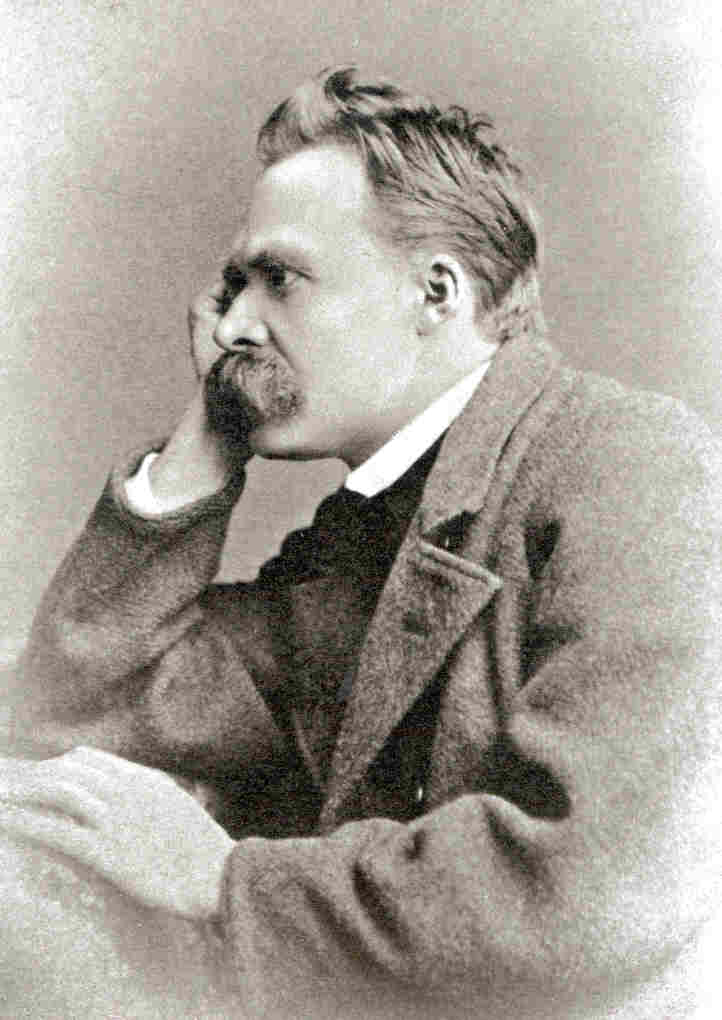
\includegraphics[height=4cm]{../../../graphics/nietzsche.jpg}
            \end{column}
            \begin{column}{7cm}
                \alert{The Doctrine of the Pathos of Distance}: Novel values only ever arise from the stable sense of power of a higher order over a lower order.
            \end{column}
        \end{columns}
\end{frame}

% section pathos_of_distance (end)

\section{The pre-moral distinction good/bad}\label{sec:the_pre_moral_distinction_good_bad} % (fold)

The rank ordering that existed in premoral aristocratic societies gave rise to the pathos of distance, the long lasting feeling of power on the part of the higher ranks of society. This sense of power involved in the aristocracy's experience of dominion over the lower classes or slaves gave rise to novel values. In particular, terms used originally as purely political designations came to be associated with what was perceived as the typical character traits of nobility. These expressions came to have a normative significance as a result of the pathos of distance, that is, the traits associated with the noble character were deemed good whereas as those character traits associated with the lower classes were deemed bad. Thus out of the rank ordered aristocratic societies and the attendant pathos of distance there arose the premoral distinction between ``good and bad''. The noble mode of valuation which arose because of a preexisting social hierarchy served itself to reinforce this hierarchy. Judgments of good and bad were not only a reflection of divisions that already existed within aristocratic societies but tended to reinforce such divisions. Thus Nietzsche speaks of rank defining modes of valuation by which he undoubtedly means the way in which the noble mode of valuation tended to reinforce the previously established social and political hierarchy.

According to Nietzsche, the noble mode of valuation grew spontaneously out of a positive sense of self. The basic concept, then is that of the good, the noble. The corresponding negative concept, the bad, is a subsequently invented concept, whose content is parasitic upon the previously established concept of the good. In devising the noble valuation of the good, the aristocrats only looked to themselves and what they perceived as there typical character traits. In devising the noble valuation of the good, the aristocracy was positively affirming what they took themselves to be. The noble, the well born felt themselves to be happy---as such they did not need to affirm themselves with essential reference to those whom they despised, the slaves. Furthermore such happiness was inextricable bound with activity and strength.

The bad, in the noble form of valuation, originally denotes the lowly the plebeian, the slaves. Subsequently the bad was itself associated with certain character traits. If the noble, the good were strong and brave and truthful, the bad were weak and cowardly and untruthful. Despite the evident contempt the higher ranks felt for the lower order, such contempt was tempered by a sense of forbearance and pity. If the noble and well born were happy, the bad were unhappy and pitable. The forbearance which tempers noble contempt is itself a sign or symptom of the positive sense of self that animates the noble form of valuation. The aristocracy did not affirm itself derivatively by a display of contempt for the slaves, rather it is out of a positive sense of self that the good arises. Nietzsche employs the platonic imagery of a pale image or shadow to describe the bad as it figures in the noble mode of valuation. Just as a shadow depends for its existence and continued stability on that which casts it, so the concept of the bad depends on the prior establishment of the concept of the good for its own content and conceptual stability. The good and the bad are not conceptually on a par---the bad derives whatever content it has in distinction from whatever was already previously established as good.

This point is worth belaboring for a couple of reasons. First of all many French commentators on Nietzsche, unduly influenced by Saussurean linguistics and structuralism, even as they look to Nietzsche as an inspiration to resist such influences, have claimed that the content attaching to the distinction between good and bad gets established by their binary opposition. However, Nietzsche is as explicit as he can be that the concept of the bad depends on and derives its content from the prior concept of the good. There is an important conceptual asymmetry between these pair of concepts. The concept of the good thus in no way itself depends on the concept of the bad as would be the case if the pair of terms derived their content from their binary opposition. 

This is not just a fussy point about Nietzsche commentary on the continent. As I indicated earlier, if considerations of the pathos of distance are to be the basis of criticism for a Christian morality that claims to be universal, Nietzsche must have in place a relatively clear distinction between positive and active valuation as exemplified by the noble form of valuation and negative and essentially reactive valuation as exemplified by Christian asceticism. The fact that the good as it figures in the noble mode of valuation is in some relatively clear sense conceptually prior to the bad is mark or symptom of the positive and active character of that valuation.

What Nietzsche means by the contrast positive, active and negative, reactive will be clearer as we discuss the slave revolt of morality, which he believes to be the source of the contemporary moral distinction between good and evil. \change

\begin{frame}<presentation>[label=slide7]
    \frametitle{The Good and the Bad}
        \begin{columns}
            \begin{column}{3cm}
                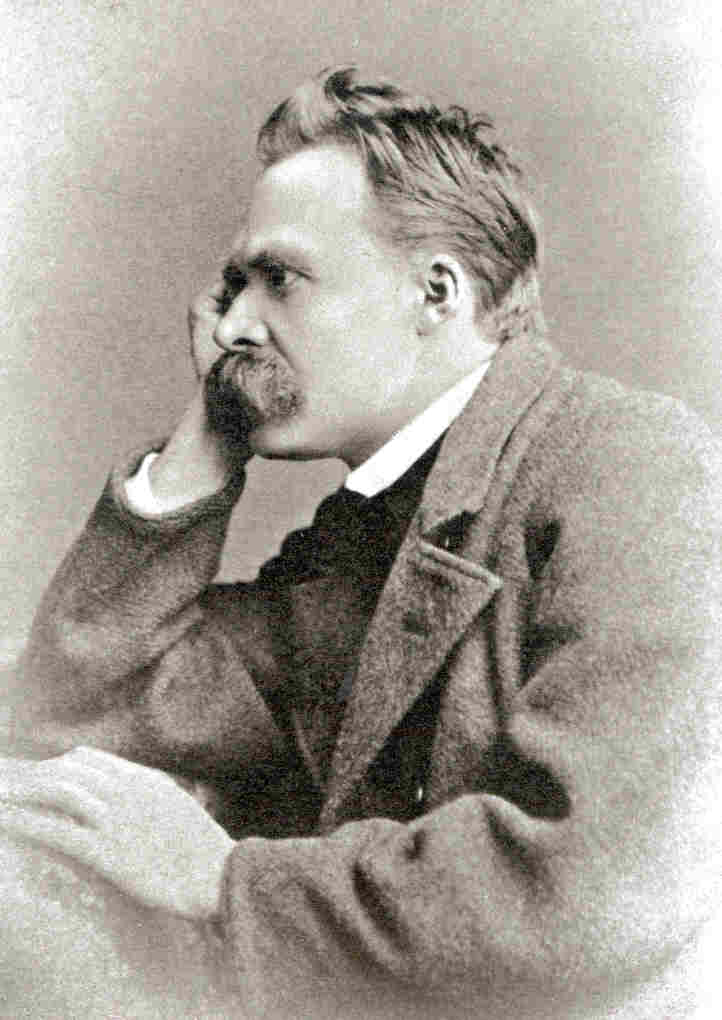
\includegraphics[height=4cm]{../../../graphics/nietzsche.jpg}
            \end{column}
            \begin{column}{7cm}
                In the pre-moral distinction between good and bad, \alert{good} is the primary notion and is the expression of a positive sense of self, and \alert{bad} is the derivative notion.
            \end{column}
        \end{columns}
\end{frame}

% section the_pre_moral_distinction_good_bad (end)

\section{The Slave Revolt}\label{sec:the_slave_revolt} % (fold)

Before we talk about the slave revolt of morality, we must get clearer about Nietzsche's metaphysics of will.

Any struggle for power involves a conflict of two or more forces. Consider, for a moment, a struggle between two forces. The outcome of such a struggle is that one of the forces dominates and the other is dominated. The dominating force, Nietzsche describes as \emph{active} and the dominated force, Nietzsche describes as \emph{reactive}. It is important to emphasize that in being dominated by an active force, the reactive force is not completely obliterated. Reactive forces continue to function by limiting or resisting the effects of the active force. So for Nietzsche, the distinction between active and reactive forces doesn't represent an intrinsic difference among forces. A force is active or reactive only in relation to another force in which it is engaged in struggle---an active force is a force that dominates and a reactive force is a force that is dominated.

There are at least two important qualitative differences between active and reactive forces. 

Reactive forces only manifest themselves in opposition to an external force, the active force that it seeks to resist. As Nietzsche puts it, reactive forces only act by reacting. In contrast, active forces manifest themselves spontaneously. Reactive forces require an opposing force against which they react. Active forces on the other hand are far more spontaneous.

Not only active forces spontaneous, but they are also form-giving. They impose a form on that which they dominate. We will see a particularly clear example of this when we discuss the second essay.

Another important distinction and a closely related one is that between positive and negative wills. As I mentioned before. Nietzsche's use of the expression will is rather elastic. Sometimes he speaks indifferently of forces as wills. Sometimes, however, he is careful to distinguish talk of wills from talk of forces. Henceforth, when we speak of the will, I will mean the regimented sense in which a will is distinguished from forces. What is this regimented sense of will which is distinguished from a force? Well, consider a struggle between two forces. The force that dominates is an active force, and the dominated force is the reactive force. Nietzsche, in the regimented sense of will, speaks of the outcome of the struggle, the contingent synthesis of opposing forces, as the will.

Just as forces can be active or reactive depending upon their relation to opposing forces, the will manifest in the struggle, the contingent synthesis of opposing forces, itself will be either \emph{affirmative} or \emph{negative}. Just as action and reaction is the expression of force, affirmation or negation is always the expression of the will to power.

A will is affirmative if it is the contingent outcome of a struggle in which active forces dominate. A will is negative if it is the contingent outcome of a struggle in which reactive forces dominate. 

Now as should be immediately evident, there is an apparent problem. How could there be a negative will? If a force is active by virtue of its relation to a force that dominates, then doesn't it follow that the reactive force, in eventually dominating in the struggle, become, by definition, active? This objection is raised by an imaginary interlocutor in section nine of the first essay. In the so-called ``epilogue of the free spirit'', the interlocutor makes just this complaint. If the reactive forces, of the slaves for instance,eventually triumph over the active fores, of the nobles for instance, hasn't the slaves become active and hence no longer reactive? In order to makes sense of the Nietzschean distinction between affirmative and negative wills, we must first answer the question, how can reactive forces triumph?

Obviously reactive forces cannot emerge triumphant in the struggle with active forces in the way that active forces do. Reactive forces cannot straightforwardly overpower the opposing force because they would become active. Reactive forces can only triumph and retain their status as reactive by more indirect means. Reactive forces triumph not by subjugating or overpowering active forces. Given the relational character of the distinction this is simply not possible. Reactive forces triumph by separating the active forces from what they can do. Reactive forces can  triumph over active forces not by overpowering them---that would simply be incoherent---but rather by dislocating an active force from what it can do. 

This is fairly abstract, but in the \emph{Genealogy} Nietzsche details a number of concrete means by which reactive forces achieve this trick of dislocation, that is, of dislocating an active force from what it can do. Indeed we will see one concrete method in the role that free will plays in the moral mode of evaluation

The distinction between active and reactive forces and positive and negative wills applies to the forces at work in an individual's will as well as forces in social and historical struggles. 

Let me make three remarks:

\begin{enumerate}
    \item The operative notion of domination need not be physical domination. The relation can take a more sublimated form. Think of how Bobby Fischer's infamous description of chess as ``psychic murder''.
    \item Human flourishing for Nietzsche is conceived by him in terms of the possession and manifestation of a positive or affirmative will. Note well that the affirmative will is characterized formally and materially. What characterizes a positive will is not what it wills, but the formal structure of the will. This is why Nietzsche can praise both Napoleon and Goethe as both possessing great will to power even though they will different things.
    \item Pathos of distance, as initially presented, is a sense of great feeling of power associated with a positive or affirmative will. Reactive forces can however, come to triumph in a struggle thus issuing in a negative will. The sense of power associated with a negative will can itself becomecreative and institute novel values. The pathos of distance associated with a negative will, the outcome of reactive forces overcoming formerly active forces that oppose it by dislocating them somehow from what they can do, Nietzsche describes as ressentiment or the spirit of revenge.
\end{enumerate}

The distance with is a prerequisite for the creation of values is the hierarchy established by opposing forces. The triumphant forces establish or constitute the higher rank where the dominated forces form or constitute the lower rank. The triumphant sense of power experienced by the dominating forces is the pathos of distance and it is out of this consciousness of power that values are created.

As should be clear, the noble mode of valuation is the manifestation is the manifestation of a positive or affirmative will, a contingent synthesis of opposing forces where active forces dominate. The characteristics associated with the noble mode of evaluation are the manifestation of this affirmative will.

The slave revolt in morality creates the moral mode of evaluation that involves the distinction between good and evil. Here we encounter the kind of bipartite structure that i described last time. We have a pre-existing practice, an aristocratic society with its noble mode of evaluation, and an opposing will that masters it and imposes upon it a novel interpretation. In the moral mode of evaluation what was formerly designated as good is now interpreted as evil. And what was formerly designated as bad is now interpreted as good. Unlike the will that governs the noble mode of evaluation, the will that establishes mastery over the noble mode of evaluation is a negative will---a will where reactive forces triumph over active forces. The sense of power associated with this negative will is the ressentiment of the slaves. The slave revolt of morality is the reinterpretation of good as evil and bad as good and arises out of the ressentiment of the slaves.

Last time I mentioned an important asymmetries in the noble and moral modes of evaluation. In the noble mode of evaluation, the good is conceptually prior to the bad, and in the moral mode of evaluation, evil is conceptually prior to the good. This is a result of the positive and negative wills the forms of evaluation manifest. In the noble mode of evaluation ``good'' is conceptually prior to ``bad'': It is the manifestation of a positive sense of self (the pathos of distance in the specific sense). In the moral mode of evaluation, ``evil'' is conceptually prior to ``good'': It is a negative reaction of the weak against the strong (ressentiment).

\begin{frame}<presentation>[label=slide8]
    \frametitle{The Slave Revolt and the Metaphysics of the Will}
        \begin{columns}
            \begin{column}{3cm}
                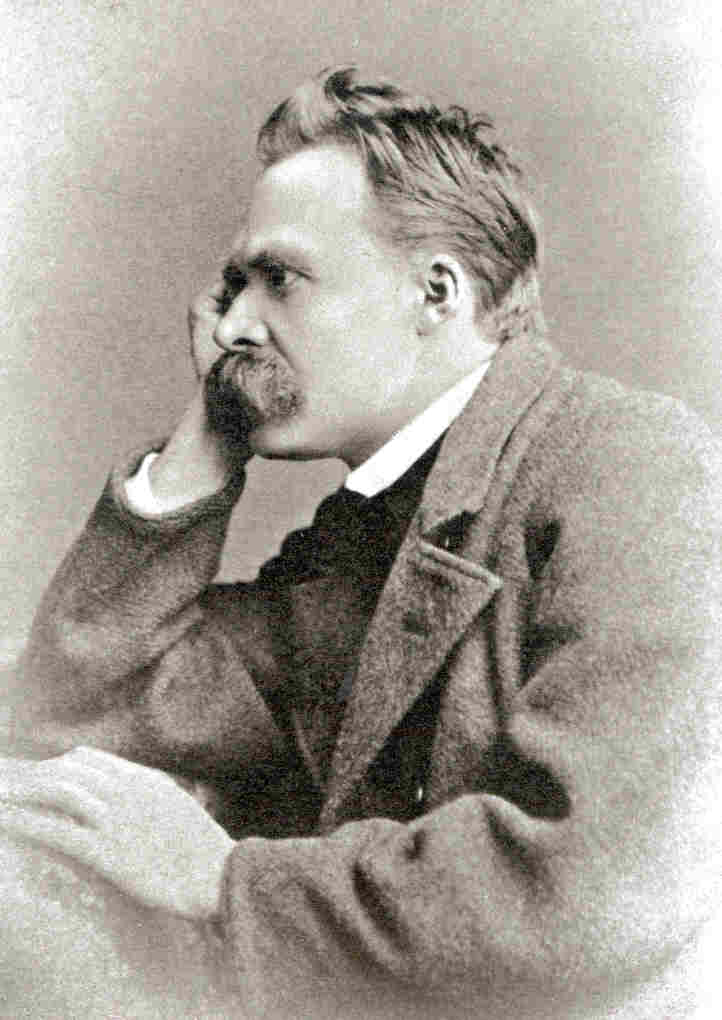
\includegraphics[height=4cm]{../../../graphics/nietzsche.jpg}
            \end{column}
            \begin{column}{7cm}
                \begin{itemize}
                    \item<1-> \alert{Active} vs \alert{Reactive} forces
                    \item<2-> \alert{Positive} vs \alert{Negative} wills
                    \item<3-> \alert{Ressentiment} as the manifestation of a negative will
                \end{itemize}
            \end{column}
        \end{columns}
\end{frame}

% 
% The slaves, motivated by ressentiment, form a novel mode of evaluation which designates ``good'' all that the nobles designated ``bad'' and designates ``evil'' all that the nobles designated good.
% 
% Ressentiment contrasts with the pathos of distance in the specific sense (the noble's stable sense of power) but is itself an instance of the pathos of distance in the general sense (the stable sense of power of a higher order over a lower order that institutes novel values).
% 
% In the noble mode of evaluation ``good'' is conceptually prior to ``bad'': It is the manifestation of a positive sense of self (the pathos of distance in the specific sense).
% 
% In the moral mode of evaluation, ``evil'' is conceptually prior to ``good'': It is a negative raction of the weak against the strong (ressentiment).
% 
% % section the_slave_revolt (end)
% 
% \section{The Priestly Subcaste}\label{sec:the_priestly_subcaste} % (fold)
% 
% Is Purity a Counterexample?
% 
% According to Nietzsche, terms originally denoting political superiority resolve over time into terms denoting moral or spiritual superiority. However, it is hard to see how “purity” originally had the required political significance.
% 
% Nietzsche claims that “purity” did originally denote a kind of political superiority. Nietzsche takes this observation as (partial) evidence of: 
% The nobles dividing into military and religious sub-castes: the warriors and the priests.
% 
% The priests deploying ritual purity to distinguish themselves from the warriors.
% 
% But isn’t this inconsistent with the hypothesis of the slave revolt? No, it is evidence of:
% 
% An internal power struggle between the warriors and the priests in which the priests make common cause with the slaves against the warriors.
% 
% % section the_priestly_subcaste (end)



\section{The Grammatical Distinction}\label{sec:the_grammatical_distinction} % (fold)

An important part of the history that leads to the establishment of the basic moral distinction between good and evil is that the weak, ``the slaves'', employed a language within which there was a contingent grammatical distinction between subject and predicate. Nietzsche believes that a commitment to free will is the elevation of this contingent linguistic distinction to the level of a metaphysical hypothesis. Notoriously Nietzsche denies that there is any such thing as free will. Such a denial must be rightly understood. His denial that the will is free doe not imply that he thinks the will is unfree, enslaved, or in bondage. Rather he holds that the whole conceptual pair  ``free/unfree '' is a fiction having no real application to the will. So in denying that the will is free, he is not asserting that it is instead unfree; rather he is rejecting the entire distinction as myth foisted on us by mistaking a contingent feature of our language as representing an essential feature of reality. Free will was the invention of weak people (slaves) who appropriated a certain contingently existing grammatical distinction to be found in Indo-European languages, the distinction between the grammatical subject of a sentence and its predicate, and transposed this distinction to the realm of metaphysics.

The grammatical subject of a sentence is an expression that denotes what the sentence is about. Thus the name ``Socrates'' is the grammatical subject of the sentence:
\begin{quote}
    Socrates is wise.
\end{quote}
and the description ``the lightning '' is the subject of the sentence
\begin{quote}
    The lightning flashed
\end{quote}
The first sentence says something about its subject, Socrates, that he is wise, and the second sentence says something about its subject, the lightning, that it flashed.
\begin{quote}
    The grammatical subject of sentence is the term used to denote thing which the sentence is about. 
\end{quote}

The grammatical subject of a sentence can be distinguished from its grammatical predicate. Where the grammatical subject of a sentence denotes the thing which the sentence is about, the grammatical predicate denotes what is said of the subject. Thus in our first sentence the grammatical predicates says of Socrates that he is wise. In our second sentence the grammatical predicate says of the lightning that it flashes.
\begin{quote}
    The grammatical predicate of a sentence is an expression that says something of the subject.
\end{quote}
In general, we can picture the grammatical distinction between subject and predicate like this:


Just as the grammatical subject of a sentence can be distinguished from the grammatical predicate, so the weak also claimed there stands an entity (the subject, agent, self, ego) behind every activity. Consider the following two sentences:
\begin{quote}
    Socrates is wise\\
    Socrates is unwise
\end{quote}
The first sentence affirms wisdom of Socrates whereas the second sentence denies wisdom of socrates. Notice though the grammatical predicates differ in each of these sentences, the grammatical subject remains the same. This, Nietzsche maintains, encourages the thought that just as one can affirm or deny that a predicate applies to a subject, the subject remaining the while the same, so similarly the self or ego stands separate from and indifferent to possible actions, so that it is a genuinely open question whether it will perform a certain action or not. That it is an open question is interpreted by the slaves as meaning that the agent has free will. The slaves then proceed to connect certain forms of moral evaluation with the correct or incorrect application of ``free will''. 

This results in the moralizing misinterpretation of language. The fact that the grammatical predicates of sentences can differ while their grammatical subjects remain the same encourages the thought that there is a self that stands separate from the actions it performs. The fact that consideration of the grammatical subject alone leaves it an open question which predicates applies to it encourages the thought that it is an open question which actions the self will perform. This open question is interpreted as free choice or freedom of the will. Moral evaluations are linked with free choice---the moral worth of a free action depends on the quality of the human choice that leads the self to perform it.

Nietzsche thinks that it is a mistake to believe that there is a separate agent standing apart from or behind actions. Such a belief is what Hume described as a projective error. In this instance it is mistakenly projecting a contingent feature of our language and projecting onto reality. There is no self or subject behind every action---all there is is the activity itself. There isn't any ``it'' that rains or thunders, just raining and thundering. An activity can be more or less powerful, even stronger or weaker, but none of this implies that there is a self distinct from the act. And insofar as the distinction between free and unfree will depends on the existence of such a subject, then none of this implies that people have free choice to be what and who they are and to act accordingly. \change

\begin{frame}<presentation>[label=slide8]
    \frametitle{The Grammatical Distinction}
        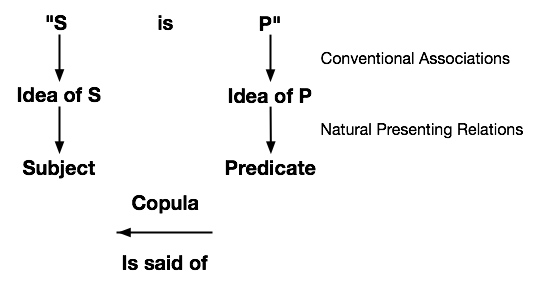
\includegraphics[width=\textwidth]{../../../graphics/subject_predicate.jpg}
\end{frame}

With the invention of free will the slaves pursued two related goals at once. First of all the fiction of free will allows them to aggrandize themselves falsely by turning their real weakness into grounds for self-congratulation. In fact they are not aggressive or successful because they are weak, but now they have the resources to give an account of this deficiency as morally meritorious. Instead of feeling weak---realizing that they can't do certain things---they feel morally superior (and thus in some sense strong) because they falsely believe that they could have done various things which they actually didn't do, but never did because they meritoriously chose never to do them.

The second goal is that of confounding and debilitating the strong as much as possible. If the slaves can succeed in lodging their fictitious notion of free will and the links it bears to certain forms of moral evaluation in the minds of those who are stronger, they will have improved the conditions of their life considerably. To the extent to which the strong come to think of themselves as having free will they will in fact begin to have a tendency to separate themselves from their actions and this will tend to make them less powerfully and spontaneously active than before, a situation advantageous to the slaves. In enforcing the distinction between free and unfree action the slaves are: 
\begin{itemize}
    \item rationalizing there own weakness in morally meritorious terms (they are not aggressive or successful because they are weak rather because they made the free, morally meritorious choice not to be)
    \item confounding and debilitating the strong (if the strong accept the distinction they will tend to separate themselves from their actions making themselves less powerfully and spontaneously active than before).
\end{itemize}

I would like to making a passing observation about the connection between Nietzsche's philosophical doctrines and his literary style. In particular, I would like to point out one way in which the Nietzsche's denial that there is any distinction between free and unfree action is implemented by a literary device that he uses. In an important passage, the first section of the preface, Nietzsche discusses how scholars are necessarily unknown to themselves. Interestingly he uses the metaphor of workers in a beehive for these workers of knowledge. Intellectual endeavor is commonly conceived to be the paradigm exemplar of free rational action (as we saw it was for Kant). The image of the beehive, and the industry of the bees, on the other hand is traditionally deployed as a metaphor for unfree non-rational instinctive activity. It is striking that Nietzsche should deploy such an image traditionally associated with unfree and non-rational action to the supposedly free and rational activity of intellectual inquiry. It should be clear that the substitution of the image of the beehive for intellectual inquiry is a calculated move on Nietzsche's part. By substituting the image of a paradigm exemplar of unfree nonrational action for the supposed exemplar of free rational action, Nietzsche is implementing his doctrine that the free/unfree distinction doesn't exist by means of this literary device. This is just one example, how Nietzsche's philosophical doctrines get embodied and indeed structure facets of the literary character of his text.

Nietzsche's discussion of the projective error involved in belief in free will also has a fairly direct connection with his critique of Christian moral practice. Remember two features of Christian asceticism that Nietzsche seeks to oppose is that (1) only free human actions are morally evaluable and (2) the moral worth of an action depends on the quality of the free choice that precedes it. If Nietzsche is right that the distinction between free and unfree action is a fiction, then crucial features of Christian moral evaluation themselves rest on a illusion. Now by Nietzsche's lights, this observation is not by itself sufficient to reject Christian morality. Nietzsche repeatedly insists with all requisite explicitness that he has no objection to illusion or fictions in and of themselves. Indeed in many places he insists that illusion is necessary for life and hence it makes no sense to be absolutely against it. Nietzsche does however make two predictions concerning the false presuppositions of traditional form of Christian morality. First that it will be increasingly difficult for moderns to fail to recognize the untruths upon which Christian morality rests and second that such recognition will cause serious social and cultural dislocation. Now many advocates of traditional morality may see in falsehood sufficient grounds for rejecting Christian morality, but that is an internal difficult for Christian morality committed as it is to a moral ideal of truthfulness. But for Nietzsche, more would have to be established since he insists, rather dramatically, that untruth is a condition for life. \change

\begin{frame}<presentation>[label=slide9]
    \frametitle{The Function of the Myth of Freedom}
        \begin{columns}
            \begin{column}{3cm}
                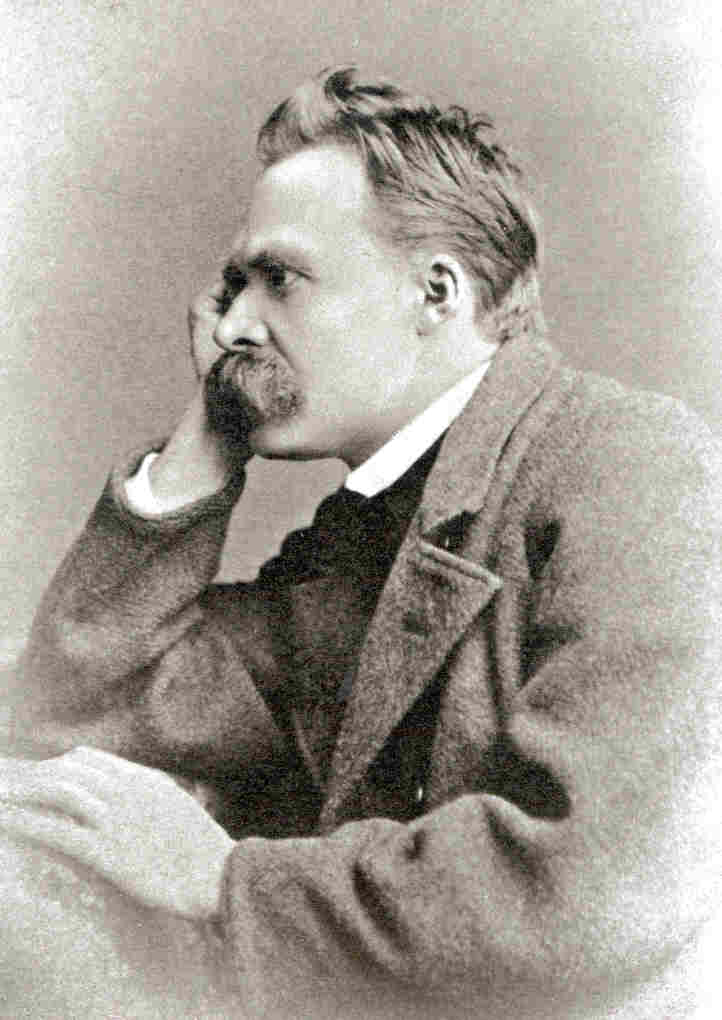
\includegraphics[height=4cm]{../../../graphics/nietzsche.jpg}
            \end{column}
            \begin{column}{7cm}
                In enforcing the distinction between free and unfree action the slaves are: 
                \begin{itemize}
                    \item rationalizing there own weakness in morally meritorious terms (they are not aggressive or successful because they are weak rather because they made the free, morally meritorious choice not to be)
                    \item confounding and debilitating the strong (if the strong accept the distinction they will tend to separate themselves from their actions making themselves less powerfully and spontaneously active than before).
                \end{itemize}
            \end{column}
        \end{columns}
\end{frame}

% section the_grammatical_distinction (end)

\section*{Summary}

\end{document}
